\newcommand{\CLASSINPUTbaselinestretch}{1.5}
\newcommand{\CLASSINPUTinnersidemargin}{25mm}
\documentclass[12pt, conference]{IEEEtran}
\usepackage{algorithmic}
\usepackage{amsfonts}
\usepackage{amsmath}
\usepackage{amssymb}
\usepackage{caption}
\usepackage{graphicx}
\usepackage{hyperref}
\usepackage{listings}
\usepackage{subcaption}
\usepackage{textcomp}
\usepackage{xcolor}

\begin{document}

\begin{abstract}
\end{abstract}

\section{Introduction}
The scanning electron microscope (SEM) is a type of microscope that produces images using signals generated from the interaction between electrons and the surface under observation. Higher resolution can be achieved compared to the traditional optical microscope, since electrons have much lower wavelength than light. An SEM can have resolution lower than one nanometre, whereas that of an optical microscope is often limited to a few hundred nanometres. This has benefited a variety of fields. For example, scientists have been using the SEM to analyse the doping density in semiconductors \cite{SEM for semiconductors} and to view changes in bacterial cells \cite{SEM for bacterial cells}.

Fig. \ref{SEM basic construction} shows the basic construction of an SEM. The electron gun generates an electron beam, which is transformed into an electron probe after passing through the condenser lens and objective lens. It is scanned across the specimen under the effect of the scanning coil. As a result of the interaction between the incident electrons and the specimen, some electrons are emitted from the specimen. These are called secondary electrons and are collected by the detector, which generates signals whose magnitude depend on the strength of the secondary electrons. The display unit produces one frame of image after each complete scan of the specimen.

\begin{figure}[htbp]
    \centering
    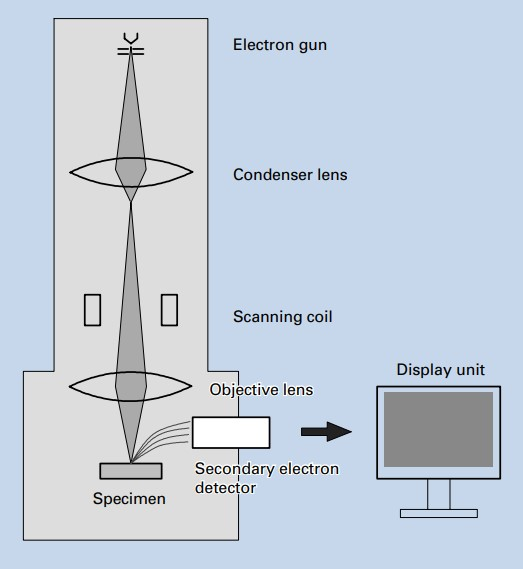
\includegraphics[width=0.45\textwidth]{Images/SEM basic construction.jpg}
    \caption{Basic construction of an SEM \cite{SEM A to Z}.}
    \label{SEM basic construction}
\end{figure}

Digital image analysis methods have been widely used in the field of SEM. For example, the fibre orientation distribution of non-woven fabrics can be determined using fast Fourier transform (FFT) and Hough transform (HT) \cite{SEM for microstructural analysis}. The FFT is an especially popular algorithm and many papers have been published on the use of it. However, due to its complexity and a lack of fast hardware, real-time analysis had largely been impossible or impractical in the past, i.e. it was only feasible to perform FFT on images off-line. In 1997, with an advanced central processing unit (CPU) --- the Pentium Pro, it was only possible to achieve a refresh rate of about 0.6 frames per second for an 8-bit 1024 $\times$ 1024 image \cite{SEM image sharpness measurement}. The enhancement of CPUs has enabled faster frame rates and more recently, the development of graphics processing unit (GPU) has taken image analysis to a different level.

The GPU was originally designed to efficiently manipulate data in order to accelerate the rendering of 3D images on displays. Depending on the position, pixels in a 3D image may require different processing to achieve effects such as lighting, blurring and fogging. This is achieved by breaking down the image into a massive number of fragments and processing each fragment individually. The processes happen independently but may share the same logical sequence of control, and this pattern is named single instruction multiple data (SIMD). A GPU consists of a large array of processing cores, with each of them using SIMD to process a block of fragments.

The characteristic of the GPU allows it to outperform central processing units (CPUs) when performing algorithms that manipulate data in parallel. Take the dot product between two vectors of size 1000 as an example, the processing cores on the GPU may be 100 times slower than the CPU, but if 1000 of them work in parallel and each computes the multiplication of one element from each vector, the overall speed will be 10 times faster. This has allowed computer vision programs that were previously impossible or computationally too expensive to build. For example, a wearable mediated reality device that make computer-generated information appear to the user as though it was anchored in the real world \cite{GPU mediated reality}.

The goal of the project is to develop software tools based on fast computation provided by the GPU, to support interactive real-time diagnosis of SEM images for the purpose of assisting the operator or automating procedures, with a focus on the use of FFT.

\section{Software aspects of the tools}
\subsection{Design principle}
Considering that the work of the project may serve as the foundation stone for many further developments, the design of the software has a strong emphasis on readability and maintainability.

\subsection{The selection of programming language}
The SEM used for the project is made by Carl Zeiss AG, which provides an application programming interface (API) that can be used for controlling the SEM and grabbing images from it. The API supports C++ and thus makes it a possible programming language for the project. Being a relatively low-level compiled language makes C++ extremely fast and useful for speed-critical applications. However, it also means that C++ has a complex syntax, which could significantly slow down development if the user does not have enough experience with it.

Considering the time scale of the project and to make development easier for people who will continue the work, Python is selected instead as the programming language, which has a much simpler syntax and is widely supported. With careful design, it has proved to be able to produce useful results despite the slower speed (see later sections).

\subsection{Modules of the software}
The software is highly modularised, which maximises readability and maintainability. This also makes it easier to translate the programs into C++ later if better performance is needed, since C++ is mostly used in an object-oriented manner. Fig. \ref{Software class diagram} shows the six main classes of the software.

\begin{figure}[htbp]
    \centering
    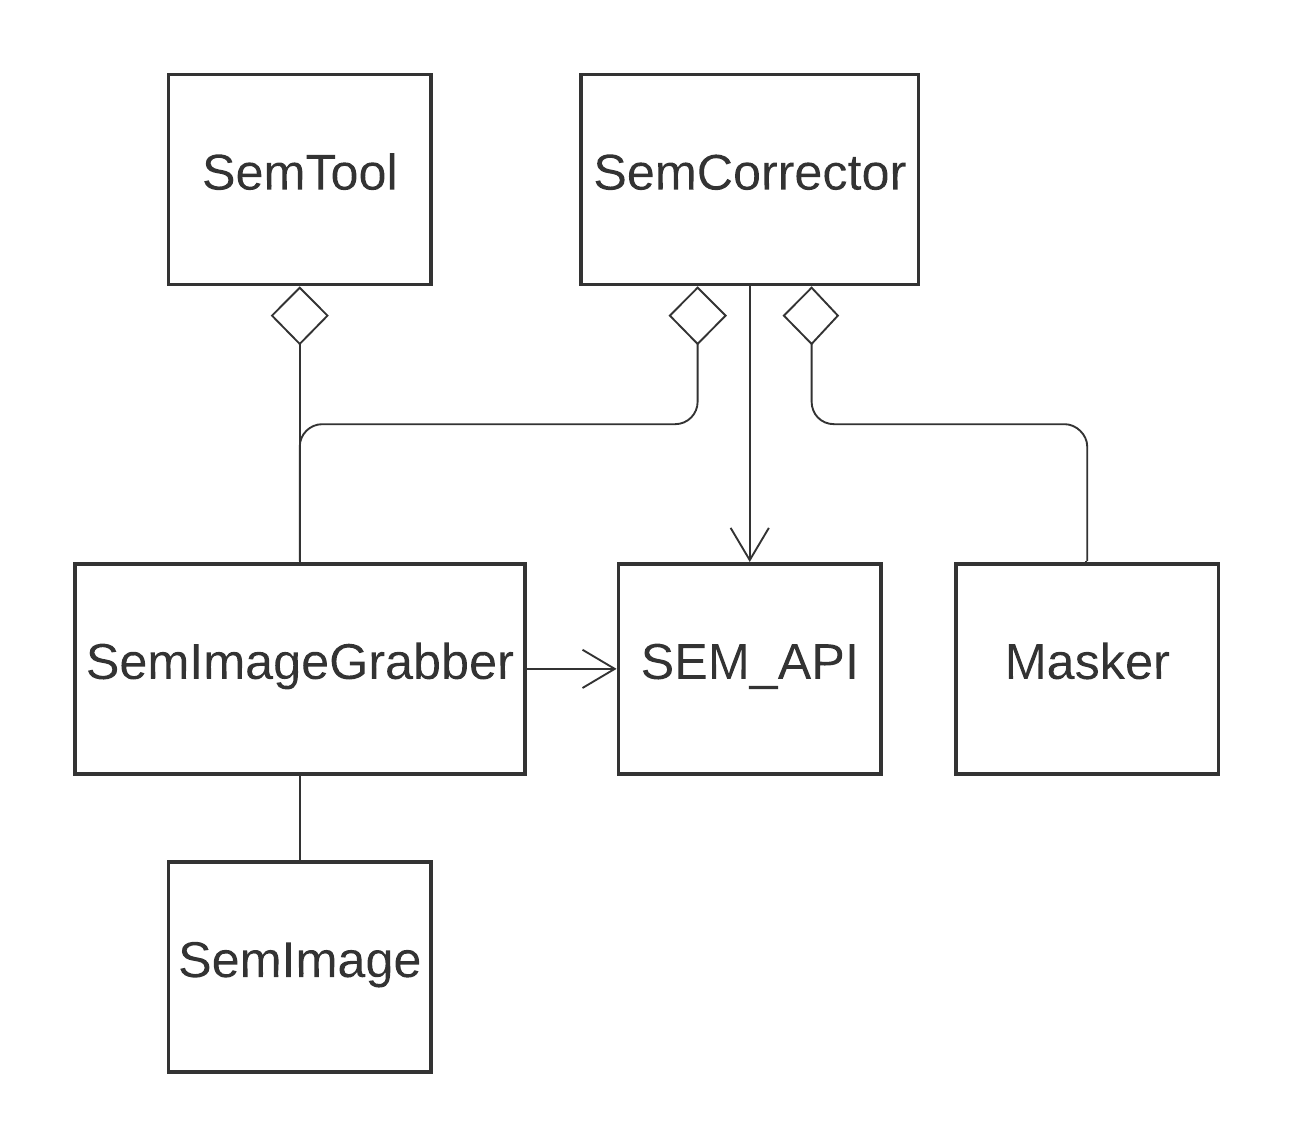
\includegraphics[width=0.45\textwidth]{Images/Software class diagram.png}
    \caption{Class diagram of the software in unified modelling language (UML)}
    \label{Software class diagram}
\end{figure}

\textit{SEM\_API} is a Python wrapper for the native SEM API written by Luyang Han, which allows the user to directly control the SEM in Python.

\textit{SemImage} encapsulates variables and methods that are directly relevant to an image taken by the SEM, and \textit{SemImageGrabber} is a helper class that helps obtain image data from the SEM and create instances of \textit{SemImage} from them. Images can be obtained in two ways:
\begin{itemize}
    \item From the SEM.
    \item From a local folder, which is helpful when the SEM is not available.
\end{itemize}
\textit{SemImageGrabber} detects if the SEM is available and decides on which way to use.

\textit{SemTool} handles the creation and rendering of the graphical user interface (GUI). Fig. \ref{Software GUI} shows a screenshot of the control panel. The push buttons open a window for the corresponding plot and the radio buttons select algorithms (see section \ref{Section histogram equalisation} and \ref{Section FFT} for detailed descriptions) to be performed on the image. The plots are shown on different windows, and can be opened and closed individually. This improves frame rate by allowing the user to close unneeded windows, and also makes it easier to add other plots later. Table \ref{Software framerates} shows that the improvement is rather significant, as rendering windows is a major time-consuming process of the software. Most of the time, the only window needed is the FFT plot, which means a refresh rate of about 16 frames per second is possible. Note that the algorithms do not slow down the rendering very much, since the computations are high optimised by the GPU.

\begin{figure}[htbp]
    \centering
    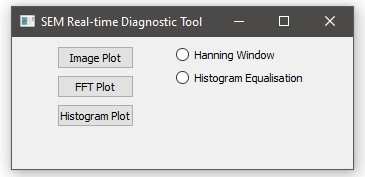
\includegraphics[width=0.45\textwidth]{Images/Software screenshot.jpg}
    \caption{Screenshot of the GUI.}
    \label{Software GUI}
\end{figure}

\begin{table}[htbp]
    \caption{Results of software framerate test}
    \begin{center}
    \begin{tabular}{|c|c|}
    \hline
    \textbf{Windows and algorithms selected} & \textbf{Framerate} \\
    \hline
    no windows, no algorithms & 10 ms \\
    \hline
    one window, no algorithms & 60 ms \\
    \hline
    three windows, no algorithms & 180 ms \\
    \hline
    three windows, two algorithms & 200 ms \\
    \hline
    \multicolumn{2}{l}{$^{\mathrm{a}}$The numbers are approximate.} \\
    \multicolumn{2}{l}{$^{\mathrm{b}}$With 8-bit grey-scale 1024 $\times$ 768 input images.} \\
    \multicolumn{2}{l}{$^{\mathrm{c}}$With Intel Core i7 and NVIDIA GeForce GTX 1060.}
    \end{tabular}
    \label{Software framerates}
    \end{center}
\end{table}

\textit{SemCorrector} implements the automatic focusing and astigmatism correction algorithm and uses a helper class \textit{Masker} to achieve fast computation (see section \ref{Section correction algorithm} for detailed descriptions). Due to the impact of the COVID-19 pandemic, the algorithm has not been fully tested, and is therefore not integrated to the GUI yet.

\section{Real-time histogram equalisation for improving image contrast}
\label{Section histogram equalisation}

\section{Real-time fast Fourier transform for evaluating image focusing and astigmatism}
\label{Section FFT}
% The quality of an SEM image is affected by aberrations. While some exist because of the fundamental properties of the microscope and are difficult to get rid of, some can be completely eliminated by adjusting relevant settings. Two important ones are focus and stigmator control, which directly affect the resolution and astigmatism of the image, respectively. Fig. \ref{SEM sample images} illustrates the effect of wrong focus and stigmator settings.

% \begin{figure}[htbp]
%     \centering
%     \begin{subfigure}{0.5\textwidth}
%         \centering
%         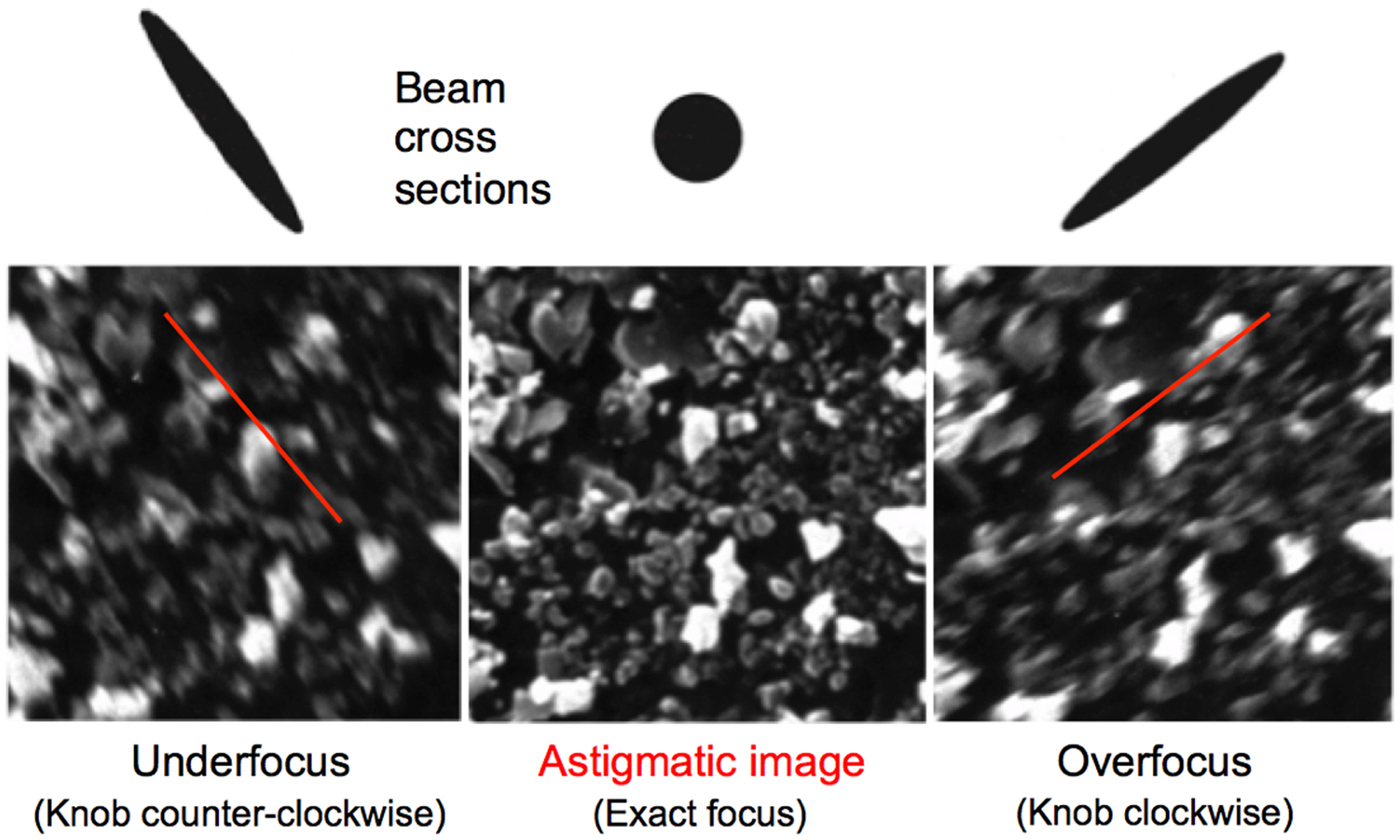
\includegraphics[width=1\textwidth]{Images/B astigmatic a.jpeg}
%     \end{subfigure}
%     \begin{subfigure}{0.5\textwidth}
%         \centering
%         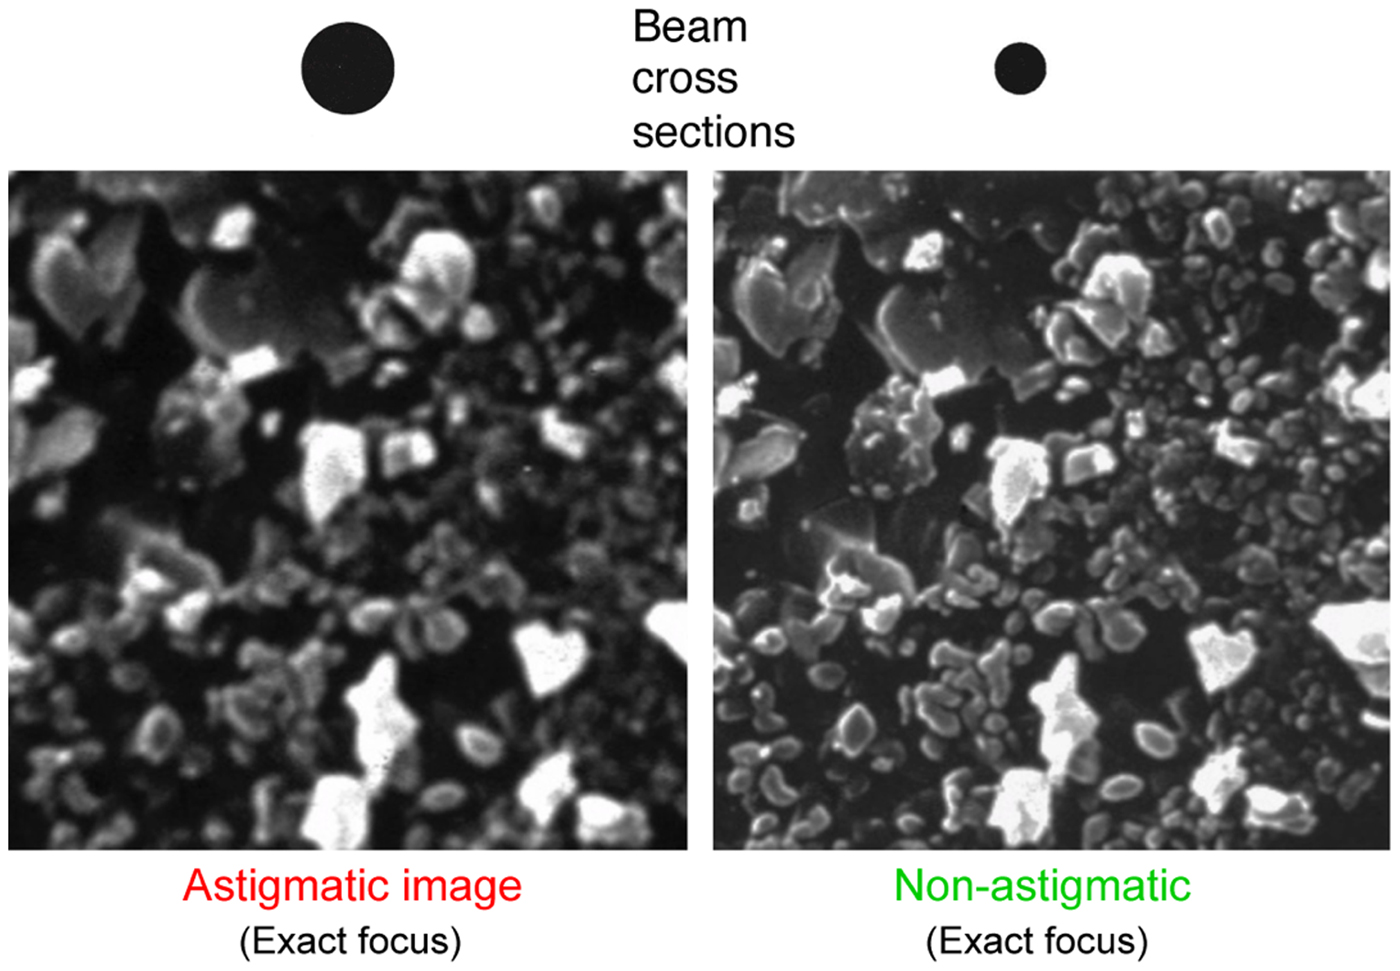
\includegraphics[width=1\textwidth]{Images/B astigmatic b.jpeg}
%     \end{subfigure}
%     \caption{Sample astigmatic SEM images \cite{SEM astigmatism correction}.}
%     \label{SEM sample images}
% \end{figure}

% Focus determines the focal point of the electron probe. When the focal point is far from the surface of the specimen, the incident electrons interact with the specimen in a larger area. As a result, spots near each other produce signals of closer magnitude. This makes the image appear blurry.

% Stigmators are used to compensate for astigmatism. Astigmatism arises due to imperfections in components of the SEM, and describes uneven focus in the electron probe, as shown in Fig. \ref{SEM uneven focus}. When the electron probe is out of focus, astigmatism makes the incident electrons interact with the specimen in an elliptical area, and thus makes the image appear stretched. When the electron probe is in focus, astigmatism makes the image appear blurry.

% \begin{figure}[htbp]
%     \centering
%     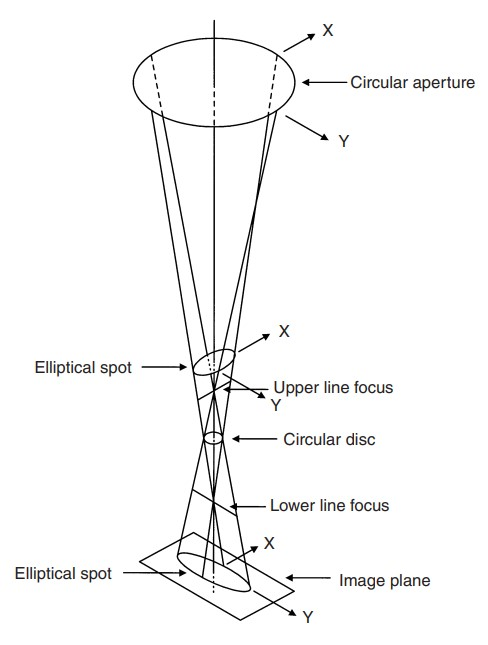
\includegraphics[width=0.5\textwidth]{Images/SEM uneven focus.jpg}
%     \caption{Uneven focus of the SEM.}
%     \label{SEM uneven focus}
% \end{figure}

% Although experienced SEM operators can often find the right settings for focus and stigmator control in a short time, it may not be as straightforward for new users. Sometimes, the surface being observed may have a complex structure and makes adjusting even harder. The complexity arises because any judgement of an image is based on what the operators see through their eyes, which is rather subjective. Intensive training and practical experience are often required for an operator to become efficient in using the SEM.

\section{Automatic focusing and astigmatism correction algorithm}
\label{Section correction algorithm}

\section{Conclusions}

\begin{thebibliography}{00}
    \bibitem{SEM for semiconductors}
    T. Agemura and T. Sekiguchi, "Secondary electron spectroscopy for imaging semiconductor materials," 2018 International Symposium on Semiconductor Manufacturing (ISSM), Tokyo, Japan, 2018, pp. 1-3, doi: 10.1109/ISSM.2018.8651171.

    \bibitem{SEM for bacterial cells}
    T. Cushnie, N. O’Driscoll and A. Lamb, "Morphological and ultrastructural changes in bacterial cells as an indicator of antibacterial mechanism of action," Cellular and Molecular Life Sciences, 2016, vol. 73, no. 23, pp. 4471-4492, doi: 10.1007/s00018-016-2302-2.

    \bibitem{SEM A to Z}
    "SEM A to Z", Jeol.co.jp, [Online], available: \url{https://www.jeol.co.jp/en/applications/pdf/sm/sem_atoz_all.pdf}. [Accessed: 18 May 2020].

    \bibitem{SEM for microstructural analysis}
    E. Ghassemieh, M. Acar and H. Versteeg, "Microstructural analysis of non-woven fabrics using scanning electron microscopy and image processing. Part 1: Development and verification of the methods," Proceedings of the Institution of Mechanical Engineers, Part L: Journal of Materials: Design and Applications, 2002, vol. 216, no. 3, pp. 199-207, doi: 10.1177/146442070221600305.

    \bibitem{SEM image sharpness measurement}
    A. Vladár, M. Postek and M. Davidson, "Image sharpness measurement in scanning electron microscopy-part II," Scanning, 2006, vol. 20, no. 1, pp. 24-34, doi: 10.1002/sca.1998.4950200104.

    \bibitem{GPU mediated reality}
    J. Fung, F. Tang and S. Mann, "Mediated reality using computer graphics hardware for computer vision," Proceedings. Sixth International Symposium on Wearable Computers, Seattle, WA, USA, 2002, pp. 83-89, doi: 10.1109/ISWC.2002.1167222.

    % \bibitem{SEM astigmatism correction}
    % C. Lyman, "Correcting Astigmatism in SEM Images," Microscopy Today, 2019, vol. 27, no. 03, pp. 32-35, doi: 10.1017/s1551929519000476.

    % \bibitem{Histogram equalisation wiki}
    % "Histogram equalization." en.wikipedia.org. \url{https://en.wikipedia.org/wiki/Histogram_equalization} (accessed May 11, 2020).

    % \bibitem{Fourier transform wiki}
    % "Fourier transform." en.wikipedia.org. \url{https://en.wikipedia.org/wiki/Fourier_transform} (accessed May 12, 2020).

    % \bibitem{Fourier transform lecture}
    % University of Oxford. (2014). 2D Fourier transforms and applications. [Online]. Available: \url{http://www.robots.ox.ac.uk/}

    % \bibitem{Fast Fourier transform wiki}
    % "Fast Fourier transform." en.wikipedia.org. \url{https://en.wikipedia.org/wiki/Fast_Fourier_transform} (accessed May 12, 2020).
    
    % \bibitem{SEM astigmatation correction algorithm}
    % K.H. Ong, J.C.H. Phang and J.T.L. Thong, "A robust focusing and astigmatism correction method for the scanning electron microscope," 1997, scanning 19: 553-563, doi: 10.1002/sca.4950190805.

    % \bibitem{Window function wiki}
    % "Window function." en.wikipedia.org. \url{https://en.wikipedia.org/wiki/Window_function} (accessed May 13, 2020).
\end{thebibliography}

\end{document}
